\chapter{Results}\label{chapter_sta}
As I argued before, discovery of recurrent behaviors from the wealth of public software artifacts can potentially 
provide new insights into the FLOSS software processes and specifically into the role of human factors through 
analyses of the motivation and constraints that modulate them. 
Thus, it is highly desirable to have an automated or semi-automated tool which implements end-to-end 
customizable workflow capable of artifacts collection, metrics extraction, and recurrent behaviors reporting.

Software Trajectory Analysis implements such workflow. 

\section{Software Trajectory Analysis overview}


\section{Previous work on STA}
The current implementation of Software Trajectory Analysis is generic by design. In fact, it can be applied 
to almost any kind of sequential software measurements that carry potentially useful information. 
This generality is granted by the STA core algorithm for characteristic patterns discovery (i.e. SAX-VSM). 
Previous STA implementations were not generic -- they were ``hard-coded'' for specific exploratory studies 
which I discuss in this section. These studies have provided valuable insights into the specificity of recurrent 
behaviors discovery from artifact measurements and into a number of aspects of system design and 
implementation.

\begin{figure}[t]
   \centering
   \includegraphics[width=150mm]{figures/STA12-schema-draft.eps}
   \caption{The Schematic overview of first two STA implementations. 
   Left panel shows a schematic representation of information flow in Hackystat: raw measurements, metadata, 
   and their abstractions seamlessly absorbed by STA, processed, and presented to the user.
   Right panel shows the information flow in a more generic, second STA implementation designed for the 
   analysis of Android OS public repository.}
   \label{fig:STA12-schema}
\end{figure}

\subsection{STA v. 1.0: mining Hackystat software telemetry streams}
The very first Software Trajectory Analysis (i.e. the pilot) implementation was designed specifically for analyses 
of the Hackystat data type called ``software telemetry''. Since software telemetry data is collected automatically 
by ``sensors'' installed at the developer's system and deployment environments, it is characterized by high 
consistency that enables unprecedented insight into performed processes, 
as I have already discussed in \ref{section_software_telemetry}. 
Effectively, by offering efficient data collection, storage, and retrieval mechanisms, and most importantly consistent, 
fine-grained data, Hackystat provided an ideal testbed for STA feasibility study.

An overview of the pilot Hackystat-based STA implementation targeting recurrent behaviors discovery is shown 
at the left panel of Figure  \ref{fig:STA12-schema}.
The pilot STA implementation has been based on two analytical techniques: the discretization of time-series with SAX \cite{sax} 
that effectively translates real-valued telemetry streams into strings, and the occurrence frequency (i.e. support) -based 
discovery of recurrent patterns.

As I have shown in \cite{csdl2-10-09}, this approach demonstrated the feasibility of recurrent behaviors discovery 
through the mining of frequently occurring symbolic patterns, i.e. time series motifs \cite{sax}. 
Consider an example of recurrent behaviors discovery shown at the Figure \ref{fig:STA1-results}, where software 
trajectories built of development effort measurements shown at the left and their clustering based on Euclidean 
distance between vectors of symbolic patterns occurrence frequencies shown at the right. Clearly, the hierarchical clustering 
process divided the set of trajectories separating two developers (\#2 and \#7) from the rest. 
Further investigation of the data revealed that these two developers demonstrated the most consistent development 
behavior (when discretized by 4 days window) as they spent considerable amounts of time working on the project almost daily
whereas the rest of the study participants did not. 
Thus, the results of STA analysis were found consistent with the ground truth.

In addition to indicating the feasibility of automated recurrent behaviors discovery through the analysis of measurements, 
the experience with the pilot system highlighted a number of issues.
The chief issue threating the external validity of the study is the small scale of the class-room experimentation that
simply does not provide an adequate coverage of the studied phenomena. 
For example, it is possible that in the above experiment some of the developers characterized by ``inconsistent 
behavior'' may simply had their Hackystat sensors mis-configured or malfunctioning, which is difficult to recognize automatically.
The second significant issue identified by the pilot STA is the problem of data mining algorithm parameters 
selection since these have to be defined as input but their proper values are difficult to guess.

Note that the pilot STA also implemented a recurrent behaviors mining workflow based on the application of 
a frequent patterns mining algorithm called Apriori \cite{citeulike:775528} to development event records collected by Hackystat. 
As I have shown in \cite{citeulike:13159603}, this approach has shown satisfactory performance. 
However, since development events are impossible (as I shall discuss in section \ref{section_understanding}) to recover from 
public software artifacts, this workflow has not been used in the following STA implementations.

\begin{figure}[t]
   \centering
   \includegraphics[width=145mm]{figures/STA1.eps}
   \caption{Results of the pilot STA study. 
   The left panel shows eight software trajectories that are Hackystat telemetry streams 
   corresponding to development effort \cite{citeulike:557296} collected from eight developers in the course of two months.
   The right panel shows a hierarchical clustering of developers by the comparison of trajectory-corresponding sets of 
   recurrent patterns discovered with SAX discretization \cite{sax}. 
   Note two distinct groups discovered by clustering: the one that contains consistent trajectories (developers \#2 and \#7) 
   and the one with less consistent trajectories.}
   \label{fig:STA1-results}
\end{figure}


\subsection{STA v. 2.0: experience with Android OS repository}
The second STA implementation has been developed targeting analyses of measurements obtained by measuring 
public software repositories artifacts.

The decision to use public software repositories in the second exploratory study has been made in order to increase its 
significance by addressing all of the essential characteristics for empirical studies based on mining software artifacts 
proposed by Gasser et al. \cite{citeulike:13058334}:  
(1) they must reflect a real-life phenomena, 
(2) provide adequate phenomena's coverage, 
(3) examine representative levels of variance, 
(4) demonstrate an adequate level of statistical significance,
(5) provide results that are comparable across projects,
(6) be reproducible. 

Unfortunately, due to the much coarser granularity and inconsistency of measurements collected from public artifacts -- 
an issue that I discuss further in this Chapter -- the original approach to data analysis based on the observed patterns 
frequency failed, and an additional exploratory study of time series mining techniques has been conducted using 
2012 MSR challenge data \cite{MSRChallenge2012} from the Android OS repository.
By experimenting with a number of time series discretization and aggregation techniques, as well as with various distance 
functions and ranking schema, I found that the Information Retrieval (IR) research field toolkit called 
Vector Space Model (VSM) \cite{citeulike:300428} that is based on \tfidf ranking schema and Cosine similarity, 
demonstrated a satisfactory performance. 

As I have shown in \cite{csdl2-11-10}, STA based on the discretization with SAX \cite{sax} and mining with VSM 
\cite{citeulike:300428}, has been found able to discover characteristic behaviors in pre- and post- release software 
trajectories constructed out of New Lines of Code change record measurements.
While the details of data processing and recurrent behaviors discovery performed within the second exploratory study will be 
discussed later in this Chapter, consider the example shown at the Figure \ref{fig:STA2-results} 
for two classes of software trajectories that reflect pre- and post- release dynamics in counts of New Lines of Code in 
the Android OS kernel repository. 
The left panel of the figure shows that it is possible to cluster characteristic behaviors corresponding to different time intervals 
where pre- and post- release behaviors are clearly separated. 
The right panel shows that by using pre- and post- release clusters centroids it is also possible to classify other time-intervals, 
which validates the discovered recurrent patterns characteristic capacity and the overall correctness of the approach.

To combat the lack of Android software repositories internal and external connectivity and the heterogeneity 
of data formats -- also the common issues in the MSR field -- in the second STA implementation I had followed the state of 
the art MSR approaches for data integration \cite{citeulike:13058334} \cite{cvsanaly}. 
In particular, similarly to a previously developed solution called softChange \cite{german04_softchange}, the second STA mirrors 
repositories and builds its own data storage facility by using the relational database engine as it is shown at 
the Figure \ref{fig:sta-assimilation}.

Note that similarly to the pilot implementation, the experience with the second STA highlighted the same problem of 
parameters selection. Moreover, the issue become even more significant since the proposed methodology was found sensitive to 
improper parameters selection. As I shall show in the next Chapter, in order to address this issue, I have explored a parameters 
optimization scheme and implemented a DIRECT-based approach \cite{citeulike:12563460} that aids in SAX-VSM 
parameters selection.

\begin{figure}[t]
   \centering
   \includegraphics[width=145mm]{figures/STA2.eps}
   \caption{An example of discovery of recurrent patterns in software trajectories constructed by measuring Android OS 
   repository source code change artifacts.
   The left panel shows the hierarchical clustering of pre- and post-release temporal interval-corresponding software 
   trajectories based on the Cosine similarity applied to ranked vectors of discovered characteristic patterns.
   The right panel shows the result of a cross-validation experiment where other pre- and post-release software trajectories 
   were classified by computing their NN similarity with previously discovered patterns.}
   \label{fig:STA2-results}
\end{figure}

\section{STA implementation}
\subsection{Data collection}
\subsection{Data transformation}
\section{Case study: PosgreSQL maintenance recurrent behaviors}
In this case study I explore the possibility of recurrent behaviors discovery from PostgreSQL - a FLOSS database that 
is developed by the PostgreSQL Global Development Group, consisting of a number of volunteers employed and 
supervised by companies such as Red Hat and EnterpriseDB \cite{postgre-contrib}.
PostgreSQL has a large number of extensions written by contributors and is available for many platforms including 
Linux, FreeBSD, Solaris, Microsoft Windows and Mac OS X.

One of the particular characteristics of PostgreSQL software process is its regular CommitFest events \cite{postgre-commitfest}.
As PostgreSQL team explains it, a CommitFest (CF) event is a ``periodic break to PostgreSQL development that focuses on patch 
review and commit rather than new development''.  Thus, it is a maintenance activity whose purpose is to promptly review 
and to respond with a feedback to development community without waiting for a major release. 

Contributors are encouraged by the core development team to submit patches into the development mailing list. Within a CF event, 
these patches reviewed, tested, and the decision for a final review and commit is made.  Typically, CFs tend to run for one month 
with a one month gap between them, however, when the core team is busy with a PostgreSQL major release, there may be several 
months without CF events followed by a ReviewFest (RF), which helps to pre-organize patches, and a CF . 

Up to date, 20 CF events were held. Typically, after reviewing and testing a patch submitted for CF developers assign it to one of the 
categories: ``Needs Review'', ``Ready for Committe'', ``Committed'', ``Returned with Feedback'', or ``Rejected''. 
While the very first CF event dealt with 66 patches, from which 37 were committed, the latest CF event had 108 patches in the review 
queue out of which 7 were marked for additional review, 14 as ready to commit, 36 were commited, and 42 were returned with feedback.

\begin{figure}[h]
   \centering
   \includegraphics[width=150mm]{postgre_commits.ps}
   \caption{PostgreSQL commit activity. Top panel: over the years the variance of activity as well as the total amount of weekly commits decreases.
   Bottom panel: there is a significant variance in commits activity throughout a year except the Christmas week.}
   \label{fig:postgre_commits}
\end{figure}

\begin{figure}[h]
   \centering
   \includegraphics[width=150mm]{postgre_churn.ps}
   \caption{An illustration of the sliding window technique from \cite{citeulike:2821475}: a time series T of length 128, 
   the subsequence $C67$ (of length $m$=16), and the first 8 overlapping subsequences extracted by a sliding window.}
   \label{fig:postgre_churn}
\end{figure}



\section{Case study: StackOverflow contributors recurrent behaviors}
\section{Case study: Android OS release recurrent behaviors}
